\documentclass[conference]{IEEEtran}
\IEEEoverridecommandlockouts
% The preceding line is only needed to identify funding in the first footnote. If that is unneeded, please comment it out.
\usepackage{cite}
\usepackage{amsmath,amssymb,amsfonts}
% \usepackage{algorithmic}
\usepackage{graphicx}
\graphicspath{ {images/} }
\usepackage{textcomp}
\usepackage{xcolor}
\usepackage{filecontents}
\usepackage{tikz}
\usepackage{pgfplots}
\usepackage{amsmath}
\usepackage{algorithm}
\usepackage[noend]{algpseudocode}


\pgfplotsset{compat=1.10}


\def\BibTeX{{\rm B\kern-.05em{\sc i\kern-.025em b}\kern-.08em
    T\kern-.1667em\lower.7ex\hbox{E}\kern-.125emX}}
\begin{document}

\title{Effective scheme against 51\% Attack on Proof-of-Work Blockchain with History Weighted Information\\
}

\author{
\IEEEauthorblockN{Xinle Yang, Yang Chen and David X. Chen}
\IEEEauthorblockA{\textit{MOAC Blockchain Tech Inc.} \\
Palo Alto, CA, USA \\
\{xinle.yang, yang.chen, david.chen\}@moac.io} 
}

\maketitle

\begin{abstract}
Proof-of-Work (PoW) is a popular protocol used in Blockchain systems to resolve double-spending problems. However, if an attacker has access to calculation hash power greater than half of the total hash power, this attacker can create a double-spending attack or 51\% attack. The cost of creating a 51\% attack is surprisingly low if hash power is abundently available. That posts a great threat to lots of PoW blockchains. We propose a technique to combine history weighted information of miners with the total calculation difficulty to alleviate the 51\% attack problem. Analysis indicates that with the new technique, the cost of a traditional attack is increased by two to three orders of magnitude.
\end{abstract}


\begin{IEEEkeywords}
Blockchain, 51\% Attack, Mining, Double spending attack
\end{IEEEkeywords}

\section{Introduction}
Developed by Satoshi Nakamoto in 2009 \cite{b1}, Bitcoin is the first decentralized public ledger system. Since then, a number of similar blockchain-based cryptocurrencies have emerged. Blockchain is a distributed data processing protocol for retaining a public distributed ledger in a Peer-to-peer (P2P) network. Transaction data is recorded in blocks, and these blocks form a linked list (i.e., chain) of blocks. Each node in the network stores and maintains an entire copy of the ledger without requiring a central authority. In blockchain-based cryptocurrencies, each block contains the hash value of the previous block, making it hard to manipulate the transactions within. Normally, a consensus protocol is used to guarantee the data integrity among the nodes of the blockchain P2P network. There are several different consensus protocols used in different types of blockchains \cite{b2}.

Proof-of-Work (PoW) is the most commonly used consensus protocol in blockchain-based cryptocurrencies. Major blockchains such as Bitcoin and Ethereum are both using different variety of PoW protocol. In PoW protocol, each node is competing to find a nonce value to produce a hash that meets a certain criteria. The difficulty of calculating such a nonce value can be calculated based on the criteria of the hash value. When such a nonce value is found, a block is generated and broadcasted to the P2P network. Depending on different varieties of protocol, peer nodes always accept the longest chain or the chain with the largest total difficulty repeatedly to continuously expand the blockchain. PoW utilizes this mechanism to determine which node has the right to seal a block. This process is also called mining.

In such a mechanism, a peer node with greater computing speed (or sometimes called hash rate power) can calculate nonce value faster than a peer node with less computing speed and thus has a higher probability of getting the right to seal a new block. However, this mechanism has a drawback. A selfish node with hash rate power higher than those of the rest nodes combined can compromise the blockchain system by causing double spending and selfish mining, etc \cite{b3}\cite{b4}. This is commonly referred to as a 51\% attack. Some studies have proposed ways to avoid such kind of attacks. Eyal and Sirer \cite{b5} in 2014 proposed a Two-Phase PoW(2P-PoW) solution preventing the formation of a mining pool with huge hash power. In this solution, the second phase PoW requires signature from the private key of the coinbase address. When the second PoW is sufficiently difficult, pool operators have to give out this private key to the pool miners in order to perform a calculation faster than all the peer nodes. Ruffing et al. \cite{b6} in 2015 proposed contracts to penalize attackers attempting a double-spending attack. Solat and Potop-Butucaru proposed ZeroBlock \cite{b7} in 2016. The mechanism in ZeroBlock requires a block to be accepted by its peers within certain time interval after the timestamp of the block. Otherwise, the block is expired. This mechanism prevents attacker nodes from selfish mining for a long period of time. J. Bae and H. Lim \cite{b8} in 2018 proposed a solution to randomly select a certain group of miners to have the right to mine the next block.

In the present paper, we introduce a new solution by utilizing a historical weighted difficulty to determine the total chain difficulty. In such a modified algorithm, a branch of blockchain has a greater total historical weighted difficulty if the miners of such a branch have a higher coverage rate in previous blocks. We demonstrate that, in reality, such an algorithm can increase the money cost and the time cost of 51\% attacks by a factor of at least two orders of magnitude.

\section{51\% attack and cost}
First, let us review the 51\% attack scheme. Assume the current hashrate is $p_o$, the attacker accumulates a greater hashrate power $p_a$ with \text{$p_a > p_o$}, and utilizes this hashrate power to compute a hidden branch $B_a$. The attacker performs double spending in two branches. The attacker then reveals hidden longer branch $B_a$ and invalidates all transactions in original branch $B_o$. The cost to launch such a 51\% attack is,
\begin{equation}
Cost=(P*R)*f*t\label{eq_cost}
\end{equation}
where $P$ is the token price, $R$ is the block reward, $f$ is the frequency of block generation speed, and $t$ stands for the duration of the attack.
For many small blockchains, the cost to perform such an attack is only hundreds or thousands of US Dollars\cite{b9}.

Another factor makes the Scenario worse is that hashrate could be easily accessible to anyone who can pay the right price. NiceHash\cite{b10} provides an open market for hashrate exchange. Anyone can easily pay with cryptocurrency to rent available hashrate to mine for the target blockchain. So an attacker can accumulate significant hashrate in short period of time to exceed the 51\% threshold. The attacker can double spend the token through a centralized exchange. The whole process only takes around 50-500 blocks. After that, attacker can release the rented hashrate and walk away with the profit. 

Most recently, Ethereum Classic\cite{b11} was attacked. Large amount of ETCs were double-spent in attack branch length ranged from 50 to 150.

\section{Historical weighted difficulty}

We propose a technique to calculate the total difficulty of a certain branch with the consideration of the miners addresses existence frequency in the previous blocks. We call this protocol Historical Weighted Difficulty based Proof-of-Work (HWD-PoW) protocol. The assumption is that in an honest blockchain branch, miners of new blocks will most likely be the miners who mined the previous blocks, and the distribution will reflect the ratio in hisotry. Furthermore, in a malicious blockchain branch, distribution of miners of new blocks will most likely be controlled by the attackers, which will be diffferent from the regular distribution of miners in the history. Therefore, when distribution of miners of mining history is considered, one can easily distinguish an honest blockchain branch from a malicious one.

Under the proposed the mechanism, branch with miners of less representation in the previous blocks will earn less weight in the total difficulty calculation. Therefore, to perform a 51\% attack, the malicious miners have two choices: either to mine a much longer branch, or to build up miner representation in the previous blocks to build up the credibility.

Now, let us look at how Historical Weight Difficulty scheme works to defend the 51\% attack. 

(a) First, record each miner’s block generation frequency for history windows $W$:
\begin{equation}
r_i=\frac{(blocks\ mined\ by\ node\ i)}{(total\ block\ number\ generated\ in\ window\ W)}\label{eq_frequency_rate}
\end{equation}
where 
\begin{equation}
    \sum_{i=0}^{n}r_i = 1
    \label{eq_frequency_normalization}
\end{equation}

(b) Each block is then signed by miner's private key. By doing this, miners will not be able to counterfeit the miner identity.

(c) When a split is detected, Historical Weighted Difficulty \text{$H\!W\!D$} is calculated for each branch at each peer node in the following way: for any unique miner $k$ in the branch $b$,
\begin{equation}
    H\!W\!D_b = H\!W_b * \!D_b = \sum_{k=0}^{l}r_k*\sum_{k=0}^{l}d_k\label{eq_hwd}
\end{equation}
where $r_k$ is the block generation frequency in the history window, $d_k$ is the difficulty of block $k$, and $l$ is the branch length.

Please note that only unique miner's generation frequency is counted. If one node mined multiple blocks, it is only counted once. This is to discourage single high hashrate miner taking over block generation, thus encourage the decentralization of mining. It also increase the difficulty of attack.

(d) Each peer node compares two different \text{$H\!W\!D$}'s from two branches. The branch with greater \text{$H\!W\!D$} will be selected.

The immediate result is clear: if the attacker just brings in temporary new hashrate power, even if the hidden branch is longer in difficulty, but the miner of the new branch is relatively new to the system, so the $r_i$ of the blocks is very low. The corresponding \text{$H\!W\!D$} will be very small compared to the original branch. No peer node in the original branch will switch to the attacker branch. This scheme can easily defend rent-and-attack case. 

If the attacker wants to make node to switch his raudulent branch, he will need to produce higher \text{$H\!W\!D$} value. The attacker needs to mine in the original branch for a while to make itself included in the history. Therefore, when it switches to hidden branch, its \text{$H\!W\!D$} will be greater. 

Suppose $p_a$ is the attacker miners' hashrate, $p_o$ is the original honest miners' hashrate.

\begin{figure}[htbp]
\centerline{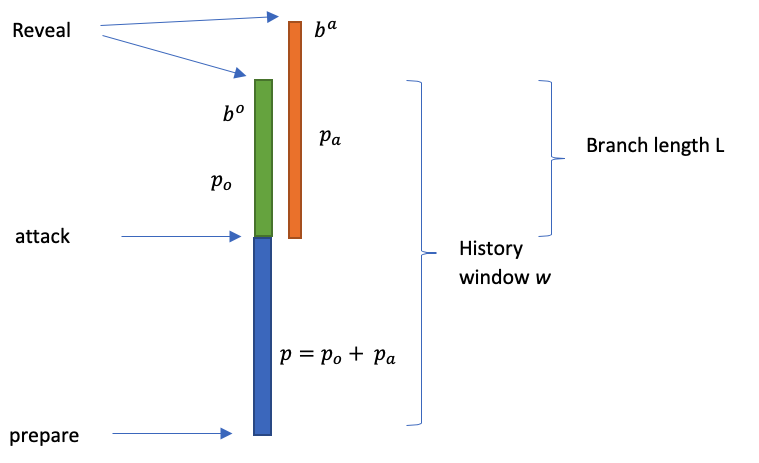
\includegraphics[width=3in]{figure.png}}
\caption{Attacker tries to attack branch $b_o$ with branch $b_a$.}
\label{fig1}
\end{figure}

The attacker needs to spend hashrate $p'$ in the original branch for a time duration $t'$. The optimum spending of $p'$ is to mine for $w/2$ period and then switch $p'$ to hidden branch at attack point show in Fig. \ref{fig1}. In order for attack to be successful, we have

\begin{equation}
    p_a > p_o\label{eq_hash_power}
\end{equation}

As a result, the revealed malicious branch $b_a$ will be longer than original branch $b_o$. 
At the reveal time, \text{$H\!W\!D$} of the original branch is,
\begin{equation}
    H\!W\!D_o = D_o * \sum_{k=0}^{l} r_{k}^{o} =  D_o * (\frac{1}{2} - \delta)\label{eq_hwd_orig}
\end{equation}
where $\delta$ is the minimal marginal difference accepted by peer node. 

So, \text{$H\!W\!D$} of the malicious branch is
\begin{equation}
    H\!W\!D_m= (\frac{1}{2} + \delta) * \frac{w-l}{w} * D_a\label{eq_hwd_mal}
\end{equation}
Therefore, we have,
\begin{equation}
    (\frac{1}{2} + \delta) * \frac{w-l}{w} * D_a> (\frac{1}{2}-\delta) * D_o\label{eq_hwd_criteria}
\end{equation}
Because $D_m$ and $D_o$ very close to each other in such a condition, we can simplify the equation to 
\begin{equation}
    (\frac{1}{2} + \delta) * \frac{w-l}{w} > (\frac{1}{2}-\delta)\label{eq_hwd_crit_simplified}
\end{equation}
and
\begin{equation}
\delta>\frac{l}{4w-2l}\label{eq_delta}
\end{equation}
To summarize, the minimal cost of the attacker is to prepare mining for $(w-l)$ duration with hashrate $p_o *(1/2+l/(4w-2l))$.

For a typical attack, $l$ needs to be around 50-500 blocks to allow token withdrawal from a token exchange. From below section, the change of miners is not very frequent. We can easily set $w > 1\ \text{month}$ to increase the history weight. With $w = 100,000$ blocks, the robustness against attack is increased by over 100 times. 

Although we cannot totally avoid 51\% attacks, we can dramatically increase the money cost and time it takes to prepare a potential attack by at least two orders of magnitude. Also, because attacker needs to spend quite a long time to prepare, the attack is much less likely to happen as the long period of time causes a lot of opportinuty cost and uncertainty.  


\section{Additional improvement schemes}

Orthogonal to above mentioned ${H\!W\!D}$ scheme, additional improvement schemes can be applied to further increase the cost of attack. 

The first approach is to post a cap of $r_i < r_c$, which means single miner can never be counted more than $r_c$ even it generates more blocks within the history window. This approach will encourage more diversified mining pool. At the same time, the miners could purposely split the mining hashrate into miltiple miners to make sure each one below $r_c$. This will circumvent the diversification requirement. However, this is still useful, as it increase the cost for attackers to maintain multiple miner accounts. 


The second approach is to post an overlap requirement between two split branches. To minimize the attack cost, attacker will focus its hashrate to the malicious branch. The overlap requires the new branch posses a certain amount of miner overlap with the old branch. Under such a condition, in order for a branch switch to happen, one needs to satisfy not only the \text{$H\!W\!D$} condition,
\begin{equation}
    H\!W\!D_a>H\!W\!D_o\label{eq_hwd_ineq}
\end{equation} 
but also, the overlap of old miners and new miners need to be greater than $s$,
\begin{equation}
    \{r_i\}\bigcap\{r_k\}>s\label{eq_overlap}
\end{equation}
where $r_i$ are the miners' frequency of original branch, and $r_k$ are the miners' frequency of attacker branch. 

Meaning, the system discourages sudden hash power switch from one set of miners to another distinct set of miners.

With such an enhanced requirement, if $s=0.25$, an attacker needs to have three times of the current hashrate within time duration $w$. This means an attacker needs to keep some hashrate in the original branch, and twice more in the malicious branch to compensate for the effect. Therefore, by introducing such a requirement, we double the time cost (and tripled the money cost) to perform an attack to the original Historical Weighted Difficulty algorithm. For higher $s$, attacker needs to spend even more hashrate than the minimal case. 

\section{$H\!W\!D$ algorithm}
In this section, we will present the algorithm to perform $H\!W\!D$ based branch selection.

Below is the pseudo code to calculate the $H\!W\!D$,

\makeatletter
\def\BState{\State\hskip-\ALG@thistlm}
\makeatother

\begin{algorithm}
\caption{Calculation of $H\!W\!D$}\label{euclid}
\begin{algorithmic}[1]
\Function{HwdCalculation}{$W, B$}
\Comment{Where W - array of historic blocks window, B - array of branch blocks}
    \State ${H\!W} = 0$
    \State $d = 0$
    \State $w = Length(W)$
    \State $l = Length(B)$
    \State Let $R[1 \ldots l]$ be new arrays
    
    \For{$i = 1$ to $l$}
    \Comment{Calculate miner appearance frequency in historic blocks window}
        \State $R[i] = 0$
        \For{$j = 1$ to $w$}
            \If {${Miner(W[j])}=={Miner(B[i])}$}
                \State $R[i] += 1$
            \EndIf
            \State $R[i] /= w$
        \EndFor
    \EndFor

    \For{$k = 1$ to ${Length(B)}$}
    \Comment{Sum Historic Weight}
        \State ${H\!W} = {H\!W} + R[k]$
    \EndFor

    \For{$k = 1$ to ${Length(B)}$}
    \Comment{Sum branch difficulty}
        \State $d = d + Diff(B[k])$
    \EndFor

    \State ${H\!W\!D} = {H\!W} * d$
\EndFunction
\end{algorithmic}
\end{algorithm}


\section{Real data statistics from Ethereum}

We picked a well-known PoW blockchain platform Ethereum. We analyzed block information of first 6,000,000 blocks, which is about 3 years mining history. The first task is to find out the distribution of miners with significant hashrate. The analysis shows that the miner distribution has a strong correlation with past history. At block \#2,000,000, \#4,000,000, \#6,000,000, the following 360 blocks were analyzed. Each miner's weight in the 360-block and weight in the 2M-block is shown in tables blew:

\begin{table}[htbp]
\caption{Ethereum block miners from 2,000,001 to 2,000,360}
\begin{center}
\begin{tabular}{lclclcl}
\hline
Miner                                      & Weight   & Amount & Weight\_in\_2M \\
\hline
0x2a65......8226 & 0.272222 & 98     & 0.239315       \\
0x61c8......0bd9 & 0.177778 & 64     & 0.049251       \\
0xbcdf......41d1 & 0.163889 & 59     & 0.023924       \\
0xea67......8ec8 & 0.116667 & 42     & 0.036458       \\
0x4bb9......1b01 & 0.063889 & 23     & 0.057752       \\
0xa42a......e84e & 0.055556 & 20     & 0.001293       \\
0x52bc......e3b5 & 0.038889 & 14     & 0.147223       \\
0x1a06......58f1 & 0.030556 & 11     & 0.004212       \\
0x6879......01da & 0.025000 & 9      & 0.023600       \\
0xd138......a31c & 0.005556 & 2      & 0.000053       \\
0xf3b9......c2fb & 0.005556 & 2      & 0.008294       \\
0xa027......e88f & 0.005556 & 2      & 0.012287       \\
0x1654......d5de & 0.002778 & 1      & 0.001272       \\
0x186a......b0f2 & 0.002778 & 1      & 0.000001       \\
0x2cb7......6402 & 0.002778 & 1      & 0.000004       \\
0x30b6......4e6d & 0.002778 & 1      & 0.002430       \\
0x40ce......f821 & 0.002778 & 1      & 0.000954       \\
0x5979......e584 & 0.002778 & 1      & 0.000116       \\
0x6caf......a46d & 0.002778 & 1      & 0.001050       \\
0x7a14......0b95 & 0.002778 & 1      & 0.001233       \\
0x9148......a49d & 0.002778 & 1      & 0.000021       \\
0x94ce......a2f7 & 0.002778 & 1      & 0.000944       \\
0x9558......7211 & 0.002778 & 1      & 0.011990       \\
0xadd8......db02 & 0.002778 & 1      & 0.000039       \\
0xd3d0......ee9d & 0.002778 & 1      & 0.001598       \\
0xdc3f......e455 & 0.002778 & 1      & 0.000340       \\
\hline
\multicolumn{4}{l}{$^{\mathrm{a}}$Total miners' weight from previous 2 million blocks is 62.57\%.}
\end{tabular}
\end{center}
\end{table}

\begin{table}[htbp]
\caption{Ethereum block miners from 4,000,001 to 4,000,360}
\begin{center}
\begin{tabular}{lclclcl}
\hline
Miner                                      & Weight   & Amount & Weight\_in\_2M\textasciitilde4M \\
\hline
0x1e99......0341 & 0.138889 & 50 & 0.079728  \\
0x2a65......8226 & 0.072222 & 26 & 0.167880  \\
0x4bb9......1b01 & 0.016667 & 6 & 0.058859  \\
0x52bc......e3b5 & 0.075000 & 27 & 0.045849  \\
0x73b8......7fea & 0.005556 & 2 & 0.007535  \\
0x829b......a830 & 0.283333 & 102 & 0.012240  \\
0x8727......87a5 & 0.005556 & 2 & 0.000331  \\
0x9435......7805 & 0.008333 & 3 & 0.003338  \\
0x9633......a11c & 0.008333 & 3 & 0.005184  \\
0xa027......e88f & 0.002778 & 1 & 0.001355  \\
0xa42a......e84e & 0.005556 & 2 & 0.033483  \\
0xa4aa......7f0d & 0.005556 & 2 & 0.003277  \\
0xa9a9......51fc & 0.002778 & 1 & 0.000911  \\
0xb293......0347 & 0.086111	 & 31 & 0.032167  \\
0xc0ea......2949 & 0.033333 & 12 & 0.072130  \\
0xea67......8ec8 & 0.236111 & 85 & 0.169016  \\
0xf3b9......c2fb & 0.013889 & 5 & 0.015585  \\

\hline
\multicolumn{4}{l}{$^{\mathrm{a}}$Total miners' weight from previous 2 million blocks is 70.89\%.}
\end{tabular}
\end{center}
\end{table}

\begin{table}[htbp]
\caption{Ethereum block miners from 6,000,001 to 6,000,360}
\begin{center}
\begin{tabular}{lclclcl}
\hline
Miner                                      & Weight   & Amount & Weight\_in\_4M\textasciitilde6M \\
\hline
0x0019......99e8 & 0.002778 & 1 & 0.000784  \\
0x1ca4......be1a & 0.019444 & 7 & 0.000904  \\
0x2a65......8226 & 0.027778 & 10 & 0.035354  \\
0x35f6......738d	 & 0.005556 & 2 & 0.000325  \\
0x4a07......a82b & 0.005556 & 2 & 0.002980  \\
0x4bb9......1b01 & 0.002778 & 1 & 0.015724  \\
0x52bc......e3b5 & 0.116667 & 42 & 0.125527  \\
0x52e4......f13c	 & 0.013889 & 5 & 0.007205  \\
0x5a0b......9c4c & 0.133333 & 48 & 0.108651  \\
0x6a7a......9b1f	 & 0.008333 & 3 & 0.008874  \\
0x70ae......e21d & 0.008333 & 3 & 0.002358  \\
0x829b......a830 & 0.127778 & 46 & 0.210382  \\
0x914d......1dcd & 0.002778 & 1 & 0.000168  \\
0x92e3......b549 & 0.002778 & 1 & 0.000822  \\
0x9435......7805 & 0.002778 & 1 & 0.007071  \\
0xb293......0347 & 0.105556 & 38 & 0.098562  \\
0xb75d......22f5	 & 0.011111 & 4	 & 0.005698  \\
0xb8f8......5453	 & 0.002778 & 1 & 0.000668  \\
0xcc16......e610 & 0.002778 & 1 & 0.002227  \\
0xd100......4fce	 & 0.002778 & 1 & 0.000470  \\
0xd380......636d & 0.002778 & 1 & 0.000002  \\
0xd438......1807 & 0.011111 & 4 & 0.000594  \\
0xd958......4012 & 0.013889 & 5 & 0.000263  \\
0xd9cf......06e3	 & 0.002778 & 1 & 0.000108  \\
0xe4bd......0649 & 0.005556 & 2 & 0.003712  \\
0xea67......8ec8 & 0.322222 & 116 & 0.259396  \\
0xf3b9......c2fb & 0.036111 & 13 & 0.023992  \\

\hline
\multicolumn{4}{l}{$^{\mathrm{a}}$Total miners' weight from previous 2 million blocks is 92.28\%.}
\end{tabular}
\end{center}
\end{table}

The total weight of 360-block miners has a strong correlation with the distribution in the history window, even the history we used is 2M blocks (about one year). The result is show in Fig.~\ref{fig2}. This reinforces our assumption that honest miner participation in the mining is relatively stable. Thus historical weight of mining history is a very valuable information we can utilize to fight against 51\% attack. We also observe that correlation of new miners with previous 2M blocks strengthened, as it indicates that Ethereum mining is going towards centralization. 

\begin{figure}[htbp]
    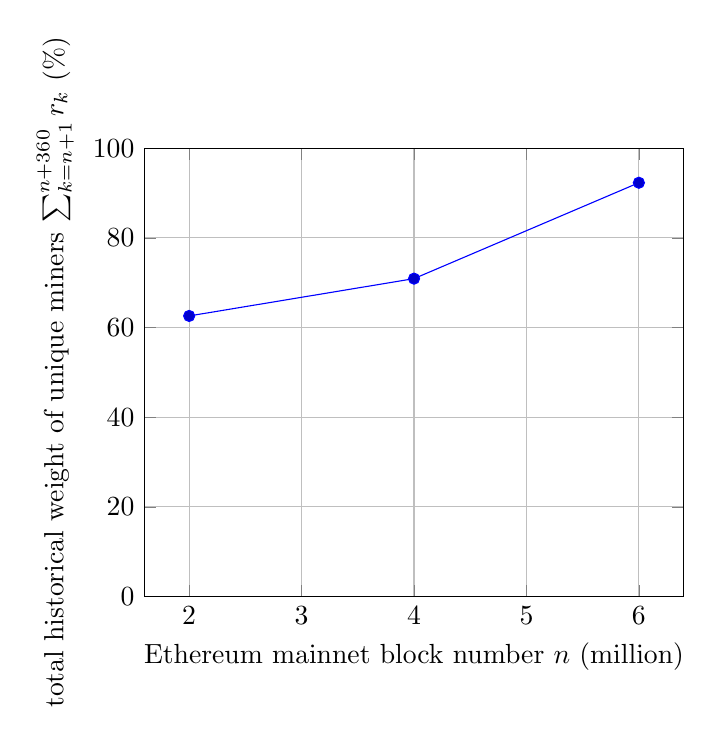
\begin{tikzpicture}
        \begin{axis}[
            xlabel={Ethereum mainnet block number $n$ (million)},
            ylabel={total historical weight of unique miners $\sum_{k=n+1}^{n+360} r_k$ (\%)},
            grid=major,
            ymin=0,
            ymax=100,
        ]
        \addplot+[sharp plot] coordinates
            {(2,62.57) (4,70.89) (6,92.28)};
        \end{axis}
    \end{tikzpicture}
    \caption{Total historical weight $H\!W$ of unique miners of the 360 new blocks from previous 2 million blocks.}
    \label{fig2}
    \end{figure}    
    
We further created an simulation to perform 51\% attack at the point of block \#2M, \#4M and \#6M, and computed the result for window length of 1M and 2M. To make it close to real case, we randomly flaged 51\% of miner in certain length back from attack point to be dishonest, which represents the attack preparation period. From the dishonest list, we picked the top 360 miners as the attack branch generator. If the attack branch HWD is higher than original branch HWD, we marked it as a successful attack. 

In the idea case, the preparation should be at least longer than the specified window. However, given the distribution of correlation, the preparation period was slightly shorter. We ran the simulation multiple time for each window to get the average accumulated cost. Here we ignored the mining reward halving effect over the time. Result is below Fig.~\ref{fig3}.

\begin{figure}[htbp]
    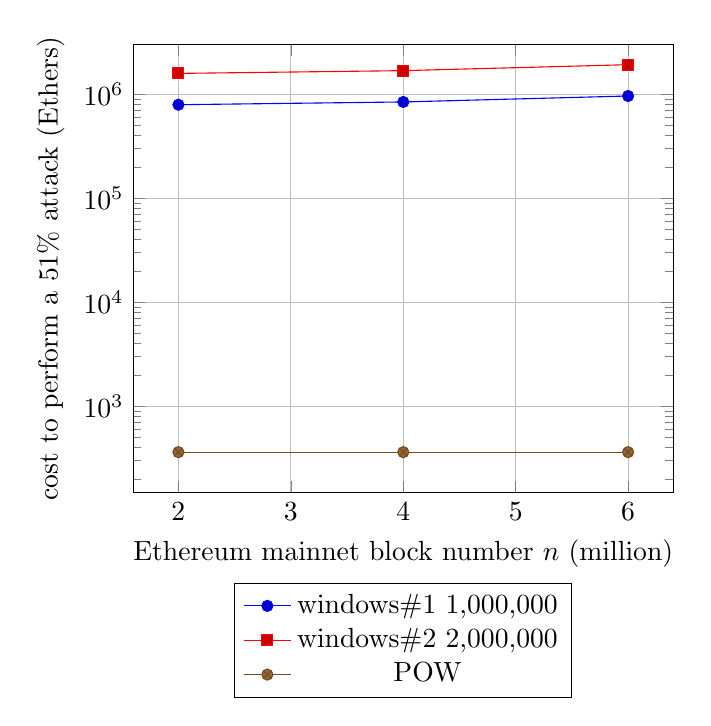
\begin{tikzpicture}
    \begin{axis}[
        xlabel={Ethereum mainnet block number $n$ (million)},
        ylabel={cost to perform a 51\% attack (Ethers)},
        ymode=log,
        ymax=3000000,
        grid=major,
        legend entries={$\text{windows\#1 1,000,000}$,$\text{windows\#2 2,000,000}$,$\text{POW}$},
        legend style={at={(0.5,-0.2)},anchor=north},
    ]
    \addplot+[sharp plot] coordinates  {(2,792148.9759) (4,841961.9944) (6,960624.7967)};
    \addplot+[sharp plot] coordinates {(2,1584297.952) (4,1683923.989) (6,1921249.593)};
    \addplot+[sharp plot] coordinates {(2,361) (4,361) (6,361)};
    \end{axis}
\end{tikzpicture}
\caption{Comparing the cost of perform a 51\% attack, HWD-PoW(1M windows, 2M windows) vs. PoW}
\label{fig3}
\end{figure}    

The result shows that with HWD scheme, the cost of attacking regular Ethereum blockchain increases by more than 1000 times, if we set the window size to be 1M and 2M. In real application, the windows could be shorter to speed up the process. We suggest window size is at least 100k, making the cost of attack is 100x more.


\section{Conclusion}
 
In this paper, we have proposed an approach to increase the cost of a successful 51\% double-spending attack on Proof-of-Work types of Blockchain protocols. The proposed approach utilizes the frequency rate of miners in history blocks and calculates the total Historical Weighted Difficulty to determine if branch switch is needed. We demonstrated in three real Ethereum Mainnet scenarios that the cost of attack is increased by more than 100 times with HWD scheme.

Our HWD scheme could be applied to all other POW based blockchains. This can improve smaller blockchain's security dramatically with easy integration. 

\section*{Acknowledgment}

This work was supported by the MOAC Foundation and MOAC Blockchain Tech Inc.

\begin{thebibliography}{00}

\bibitem{b1} S. Nakamoto,``Bitcoin: A peer-to-peer electronic cash system," 2008.
\bibitem{b2} Z. Zheng, S. Xie, H. Dai, X. Chen, and H. Wang, ``Blockchain challenges
and opportunities: A survey," Internat. J. Web Grid Serv., 2016.
\bibitem{b3}M. Conti, S. Kumar E, C. Lal, and S. Ruj, ``A survey on security and privacy issues of Bitcoin," arXiv preprint arXiv:1706.00916, 2017.
\bibitem{b4} Eyal, I. and Sirer, E.G. (2014) ``Majority is not enough: Bitcoin mining is vulnerable", Proceedings
of International Conference on Financial Cryptography and Data Security, Berlin, Heidelberg,
pp.436–454.
\bibitem{b5} I. Eyal and E. G. Sirer, ``How to disincentivize large Bitcoin mining pools," 2014.
\bibitem{b6} T. Ruffing et al., “Liar, liar, coins on fire!: Penalizing equivocation by loss of Bitcoins," ACM Conf. Comput. Commun. Secur., Oct. 2015.
\bibitem{b7} S. Solat and M. Potop-Butucaru,``ZeroBlock: Preventing selfish mining in Bitcoin," arXiv preprint arXiv:1605.02435, 2016.
\bibitem{b8} J. Bae and H. Lim, ``Random Mining Group Selection to Prevent 51\% Attacks on Bitcoin," 2018 48th Annual IEEE/IFIP International Conference on Dependable Systems and Networks Workshops (DSN-W), Luxembourg City, 2018, pp. 81-82. 
doi: 10.1109/DSN-W.2018.00040
\bibitem{b9} PoW 51\% attack cost, https://www.crypto51.app
\bibitem{b10} NiceHash - Largest Crypto-Mining Marketplace to sell or purchase hash power, https://www.nicehash.com/
\bibitem{b11} Deep Chain Reorganization Detected on Ethereum Classic (ETC), https://blog.coinbase.com/ethereum-classic-etc-is-currently-being-51-attacked-33be13ce32de

\end{thebibliography}
\vspace{12pt}
\color{red}

\end{document}
